\documentclass{article}
\usepackage[final]{nips_2017}
\usepackage[utf8]{inputenc} % allow utf-8 input
\usepackage[T1]{fontenc}    % use 8-bit T1 fonts
\usepackage{hyperref}       % hyperlinks
\usepackage{url}            % simple URL typesetting
\usepackage{booktabs}       % professional-quality tables
\usepackage{amsfonts}       % blackboard math symbols
\usepackage{nicefrac}       % compact symbols for 1/2, etc.
\usepackage{microtype}      % microtypography
\usepackage{graphicx}
\title{Make yourself into a work of art}

\author{
  Kiah Hardcastle \\
  Neuroscience PhD Program \\
  Stanford University\\
  \texttt{khardcas@stanford.edu} \\
  %% examples of more authors
   \And
  Julie Makelberge \\
  Graduate School of Business \\
  Stanford University \\
  \texttt{juliemkb@stanford.edu} \\
  %% \AND
  %% Coauthor \\
  %% Affiliation \\
  %% Address \\
  %% \texttt{email} \\
  %% \And
  %% Coauthor \\
  %% Affiliation \\
  %% Address \\
  %% \texttt{email} \\
  %% \And
  %% Coauthor \\
  %% Affiliation \\
  %% Address \\
  %% \texttt{email} \\
}

\begin{document}
% \nipsfinalcopy is no longer used

\begin{center}

\includegraphics[width=3cm, height=0.7cm]{CS230}
\end{center}

\maketitle

\begin{abstract}
In this paper, we present a method by which one can integrate a person's face into an artistic painting containing a face. For example, given a headshot and an artistic portrait, this method will inpaint the face in the headshot photo into the portrait face, while retaining the artistic style of the painting. To accomplish this task, we drew upon existing techniques of face swapping and portrait-specific neural style transfer. This approach builds on this previous work in several ways. First, while a number of applications have focused on face swapping in recent years, they have generally been applied to photograph images with a similar style. Second, the few methodologies that have used neural style transfer combined with face-swapping have transfered the transfered the style of the artistic image to the headshot image, without putting the newly-styled headshot image into the artistic image. Thus, our approach is novel in that we aim to retain the style and pose of the original work of art's face, regardless of the pose of the supplied image, and  reintroduce the face in the work of art as a whole. 
\end{abstract}

\section{Introduction}  
With the advent of neural style transfer in 2015 \cite{gatys2015neural}, and generative adversarial networks in 2014 \cite{gan2014}, altering artwork, or even generating novel artwork, via neural networks has become a topic of high interest in both the computer science and art communities. For example, in October 2018, an AI-generated piece of artwork sold for nearly half a million dollars. Over the last year, AI-generated art was featured in art galleries in San Francisco ("DeepDream") and New York City ("Faceless Portraits Transcending Time"). Understanding how neural networks can alter or generate art will be an important component of understanding how AI performs activities previously thought to be restricted to humans. Here, we aim to understand and implement these techniques in order to alter an existing previous piece of artwork in a personalized manner. 

In our method, we alter an existing piece of artwork by injecting the content of a headshot photograph into an original piece of art. Specifically, our framework takes two images: 1. a photograph image containing a face and 2. an artistic photo containing a face, and returns one image: a new version of the original artistic photo, but with the face replaced. The replaced face is in the same pose, and in the same style, as the original artistic face, but the content of the face is drawn from the photographed face. To accomplish this task, we combine face-swapping with neural style transfer techniques. Our approach differs from traditional face-swapping methods in that it deals with images of fundamentally different style (artistic images versus photographs), and differs from traditional neural style transfer methods in that it requires face-swapping, and replaces a subset of the content (i.e. just the face) of the artistic image. This technique would be valuable in the world of generative art as it allows different and personalised renderings of the same types of art work. 

\section{Related work}

In our project, we implement neural style transfer (NST) to imbue the face in the photograph image with the texture of the artistic photo. NST is the technique of using deep neural networks to transfer the style of a given reference image to the content of another. Prior to 2015, style transfer was accomplished with classic image processing techniques such as histogram matching \cite{neumann2005color}. However, in 2015, Gatys et al. introduced a novel technique that leverages the power of Convolutional Neural Networks (CNN) to emulate famous painting styles in natural images \cite{gatys2015neural}, \cite{gatys2016}. In their seminal paper, they proposed to capture the style and content elements of images by using the activations of different layers of a pre-trained CNN. In many modern works, including this project, VGG-19 is used \cite{Simonyan14c}. In this technique, an image is learned via an optimization procedure in which the style-activations of the learned image attempt to match the style-activations of the style image, while the content-activations of the learned image attempt to match the content-activations of the content image. 

Their work has inspired a number of new neural transfer algorithms, ranging from general models such as the work of Li and Wand \cite{li2016combining} that combined generative Markov random field models with deep convolutional neural networks, to highly specialized domain-specific models such as Jiang and Fu's Fashion style generator \cite{jiang2017fashion}. While general models have shown great potential in a large number of applications, they generally introduce visual artifacts. These artifacts can be striking in faces, especially since humans are sensitive to face irregularities. Several works have attempted to address these artifacts. In 2014, Shih et al., developed an approach that transfered style between headshot portraits by first finding a pixel-to-pixel correspondence between images, and then decompose each image into "Laplacian stacks" that they match between images \cite{Shih2014}. However, this method only works when transfering style between photographs. In 2016, Selim et al. introduced an approach that first aligns the artistic and photograph faces, and then learns a new image via NST with an altered set of content activations \cite{selim2016painting} (described in detail below). This technique works well for portrait-specific NST, but does not replace the face in the artistic image. In 2017, Liao et al. developed another approach using "deep image analogy" \cite{Liao2017}. Briefly, this approach takes two semantically-related photos (e.g. images of people), finds "deep features" by plotting the CNN representations of each image in a feature space, finds the nearest neighbor field using the PatchMatch algorithm to establish a correspondence between the images, and then uses this correspondence to generate new images. While the approach appears to work well, we found the method difficult to parse. 

In this work, we implement, and then build upon, the portrait-specific NST as performed in Selim et al., 2016. Beyond implementing NST, accomplishing this task requires us to properly align the faces, and then accurately replace the artistic face with the newly-styled photograph face. Much work has been done recently in face alignment. In particular, in 2018 Zhu et al. developed a method to label landmarks in 3d for faces in a wide range of poses \cite{zhu2019face}. However, here we use a more standardized approach of detecting faces, detecting landmarks on faces, and warping faces using a combination of OpenCV and dlib \cite{opencv_library}, \cite{dlib09}. By combining methods from \cite{selim2016painting},\cite{opencv_library}, and \cite{dlib09}, we are able to accomplish our task.

\section{Dataset and Features}

Implementation of our method requires several pre-trained networks: VGG-19 trained on ImageNet \cite{Simonyan14c}, an OpenCV Haar-feature face detector trained on a dataset of faces \cite{opencv_library}, and a dlib landmark detector trained on an iBUG 300-W face landmark dataset \cite{dlib09}. However, once these pre-trained networks are downloaded, the rest of our implementation does not require training or testing datasets. To gather headshot photo images and artistic portraits, we used our own headshots, images from Google Image, and images from \cite{selim2016painting} (examples shown in Figure 1). The resolution of images in our dataset ranged from roughly 200 x 200 pixels to 800 x 800 pixels. If more images are needed in the future, one can also draw from the Web Gallery of Art \cite{WebGallery} and the celebA dataset \cite{liu2018large}.

\begin{figure}[ht]
  \begin{center}
    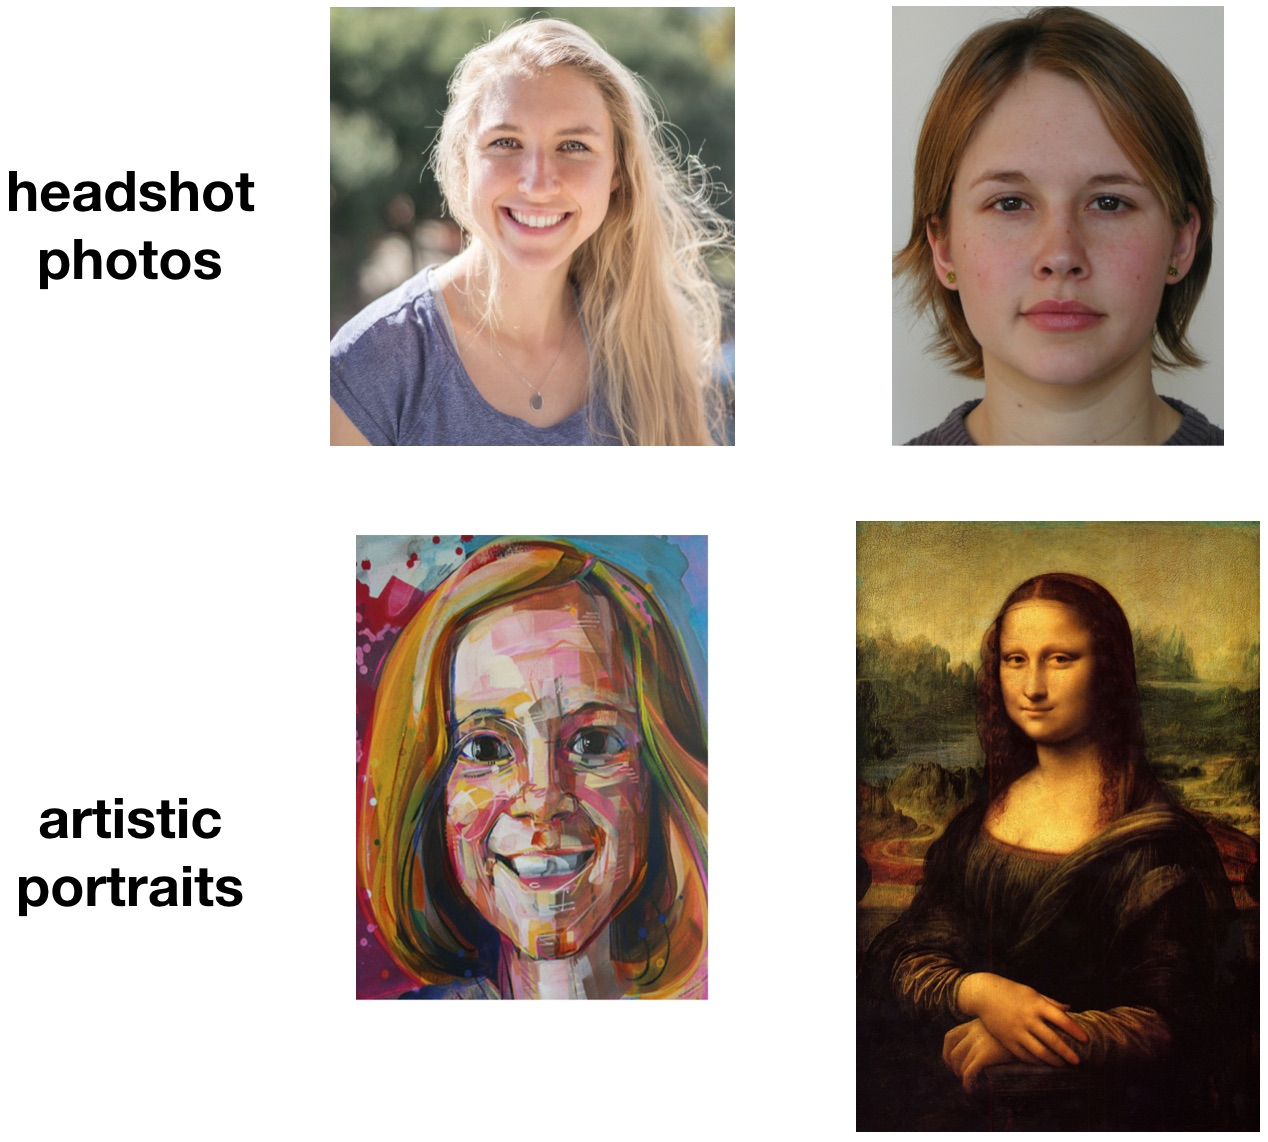
\includegraphics[width=.45\textwidth]{example_images.jpg}
    \caption{Examples of headshot photographs and artistic portraits} \label{fig:examples}
  \end{center}
\end{figure} 

\section{ Methods }

Replacing an artistic face with a photographed face requires three main steps. First, the 

Solving this task requires solving several sub-problems: cropping faces, warping faces so that promiment landmarks are location-matched, performing neural style transfer in order to transfer the style of the artistic painting to the photographed face, and seamlessly replacing the face in the artistic painting with a new face. 

\subsection{Face alignment}

The first step in our pipeline is to identify the face in both images (image A and image B), and generate new images A' and B', which are the cropped-out face of images A and B respectively. To accomplish this, we implemented an open-source face recognition from the OpenCV package. Following the procedure detailed in the Medium blogpost \cite{Medium}, we used Haar Feature-based Cascade Classifiers to detect the bounding box of the face. In brief, Haar features are similar to the filters in a CNN, but different in that they are not learned during training - they are pre-determined. Each filter can be used in a classifier to determine whether or not a face is present in a bounding box of the image. While the classification based on one Haar filter is not great, combining the output of many filters (e.g. through boosting) will return a relatively good classification. The OpenCV implementation organizes the features into a cascade, so that a lot of filters are "tried" if the image within the bounding box seems promising (i.e. early filters classify the image as a face). The OpenCV implementation contains pre-trained filters for faces, which we can load and then use to detect face regions within an image (see code in the github).

The second step in our pipeline is to properly align the faces so that the pose of the face is similar between the two images. Specifically, we want face B to be in the same pose as face A - e.g. the major face landmarks (eyes, nose, mouth, chin) should be in similar locations. To accomplish this, we must first identify important landmark features in both images, and then apply a transformation to get face B in the same pose as face A. In order to identify salient landmarks, we used the dlib face detection and landmark identification package, and based our code off of a github repository \cite{dlibgit}. An example of the output of this procedure is given below

We will then implement a function that will transform the headshot photo into the same pose as the artistic photo by applying a transformation that will align the landmark points. While we have not completed this yet, we plan on completing this step for our final deliverable. 

 Haar features are similar to the filters in a CNN, but different in that they are pre-determined. Each filter is used in a classifier to determine whether or not a face is present in a bounding box of the image, and the output of many filters is combined to achieve good classification accuracy (e.g. through boosting). The OpenCV implementation organizes the features into a cascade, so that a lot of filters are tried if the image within the bounding box seems promising. 

\subsection{Portrait Neural Style Transfer}

While ultimately we feel that the third method is the most promising, as it is focused on style transfer of portraits, thus far we have focussed on more traditional neural style transfer on the cropped images of face A and face B given our time constraints and the availability of pre-trained CNN weights. We are currently working with two implementations of Neural Style Transfer. In the first, we altered the code that was used in the Coursera course to perform neural style transfer on our two images. In this method, we generate a new image B' with the content of face B and in the style of face A. To do this, we minimize the following loss function:
\[
J(G)=\alpha J_{content}(B,B')+\beta J_{style}(A,B')
\]
where
\[
 J_{content}(B,B') = \frac{1}{4n_Hn_Wn_H} \sum_{all} (a(A) - a(B'))^2
\]
and 
\[
 J_{style}(B,B') = \sum_l  \lambda_l \frac{1}{(2n_Hn_Wn_H)^2} \sum_{ij} (B'_{ij}(A)^{(l)} - B'_{ij}(B')^{(l)})^2
\]

where $a(A)$ are the activations of single layer of a pre-trained VGG-19 network with the content image as input, $a(B')$ are the activations of the same layer of the VGG-19 network with the newly generated image put through, $B'_{ij}(S)^{(l)}$ is the Gram matrix of activations of a single layer ($l$) of the same network when the style image is used as input, and finally $B'_{ij}(G)^{(l)}$ is the Gram matrix of activations of a single layer of the same network when the newly generated image is used as input. Minimizing this loss function by altering the pixels in the generated image will result in a new image that contains the content of the content image, and the style of the style image. 

While we were able to successfully perform neural style transfer using our code from the homework, we found another implementation of the same algorithm that gave us a much better output \cite{NeuralStyleTranferGithub}. The result of this implementation is shown below in Figure 3:

\subsection{Face replacement}

Finally, we must replace the original face A with the new, properly aligned face C. This task contains two components: first, we replace the pixels within the original bounding box in image A with the new image B'. Second, we must then smooth the boundary between in the inpainted pixels and the border. The first step of this procedure is quite easy. To do the second step, we will remove the area around the bounding box of the face (i.e. the boundary between the new image and the old image), and then use methods of inpainting in order to fill in the boundary. 



\section{Experiments/Results/Discussion}

You should also give details about what (hyper)parameters you chose (e.g. why did you
use X learning rate for gradient descent, what was your mini-batch size and why) and how
you chose them. What your primary metrics are: accuracy, precision,
AUC, etc. Provide equations for the metrics if necessary. For results, you want to have a
mixture of tables and plots. If you are solving a classification problem, you should include a
confusion matrix or AUC/AUPRC curves. Include performance metrics such as precision,
recall, and accuracy. For regression problems, state the average error. You should have
both quantitative and qualitative results. To reiterate, you must have both quantitative
and qualitative results! If it applies: include visualizations of results, heatmaps,
examples of where your algorithm failed and a discussion of why certain algorithms failed
or succeeded. In addition, explain whether you think you have overfit to your training set
and what, if anything, you did to mitigate that. Make sure to discuss the figures/tables in
your main text throughout this section. Your plots should include legends, axis labels, and
have font sizes that are legible when printed.

\section{Conclusion/Future Work }
Summarize your report and reiterate key points. Which algorithms were the highestperforming?
Why do you think that some algorithms worked better than others? For
future work, if you had more time, more team members, or more computational resources,
what would you explore?

\section{Contributions}
The contributions section is not included in the 5 page limit. This section should describe
what each team member worked on and contributed to the project.

\medskip
\small

\bibliography{References}
\bibliographystyle{plain}

\end{document}